\documentclass[tikz]{standalone}
 
\usepackage{pgfplots}
\pgfplotsset{compat=1.14}


\begin{document}
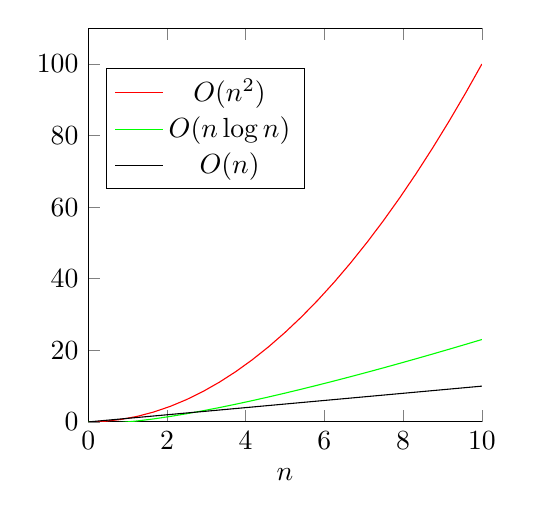
\begin{tikzpicture}
\begin{axis}[
%width=10cm,height=8cm,
width=5cm,height=5cm,
ymin =0,
xmin =0,
xmax = 10,
domain= 0:10,
scale only axis,
axis y line*=left,
xlabel={$n$},
ylabel style = {align=center},
tick label style={/pgf/number format/fixed},
ylabel={},
legend style={at={(0.55,0.9)}}
]
%\addplot table [x=size, y=insertion-sort, column sep=tab] {output.dat}; \addlegendentry{ins};
%\addplot table [x=size, y=selection-sort, column sep=tab] {output.dat}; \addlegendentry{sel};
%\addplot table [x=size, y=mergesort,      column sep=tab] {output.dat}; \addlegendentry{mer};
%\addplot table [x=size, y=quicksort,      column sep=tab] {output.dat}; \addlegendentry{qsort};

\addplot [red,mark=none]{x * x}; \addlegendentry{$O(n^2)$};
\addplot [green,mark=none]{x * ln x}; \addlegendentry{$O(n \log n)$};
\addplot [black,mark=none] {x};  \addlegendentry{$O(n)$};

\end{axis}
%
\end{tikzpicture}
\end{document}

